\documentclass[../MATLAB_Primer.tex]{subfiles}
\begin{document}

MATLAB's built-in App Designer allows users to easily create functional and interactive Graphical User Interfaces (GUIs). The App Designer can be accessed with the following command:
\\ \\
\textit{input:}
\begin{lstlisting}
>> appdesigner
\end{lstlisting}
\textit{output:}
\begin{center}

\end{center}

\subsection{App Designer Layout}
The App Designer has two separate views that you can toggle between while creating your GUI: the Design View and the Code View.
\subsubsection{Design View}
As you can see in Figure \ref{fig:designViewLayout}, the Design View features three separate sections, the Component Library, the Canvas, and the Component Browser. Available components are shown in the Component Library and can be drag and dropped to the Canvas to add them to the GUI. Once a component is added to the GUI it will appear in the Component Browser with information regarding its appearance and functionality.
\begin{figure}[H]
    \centering
    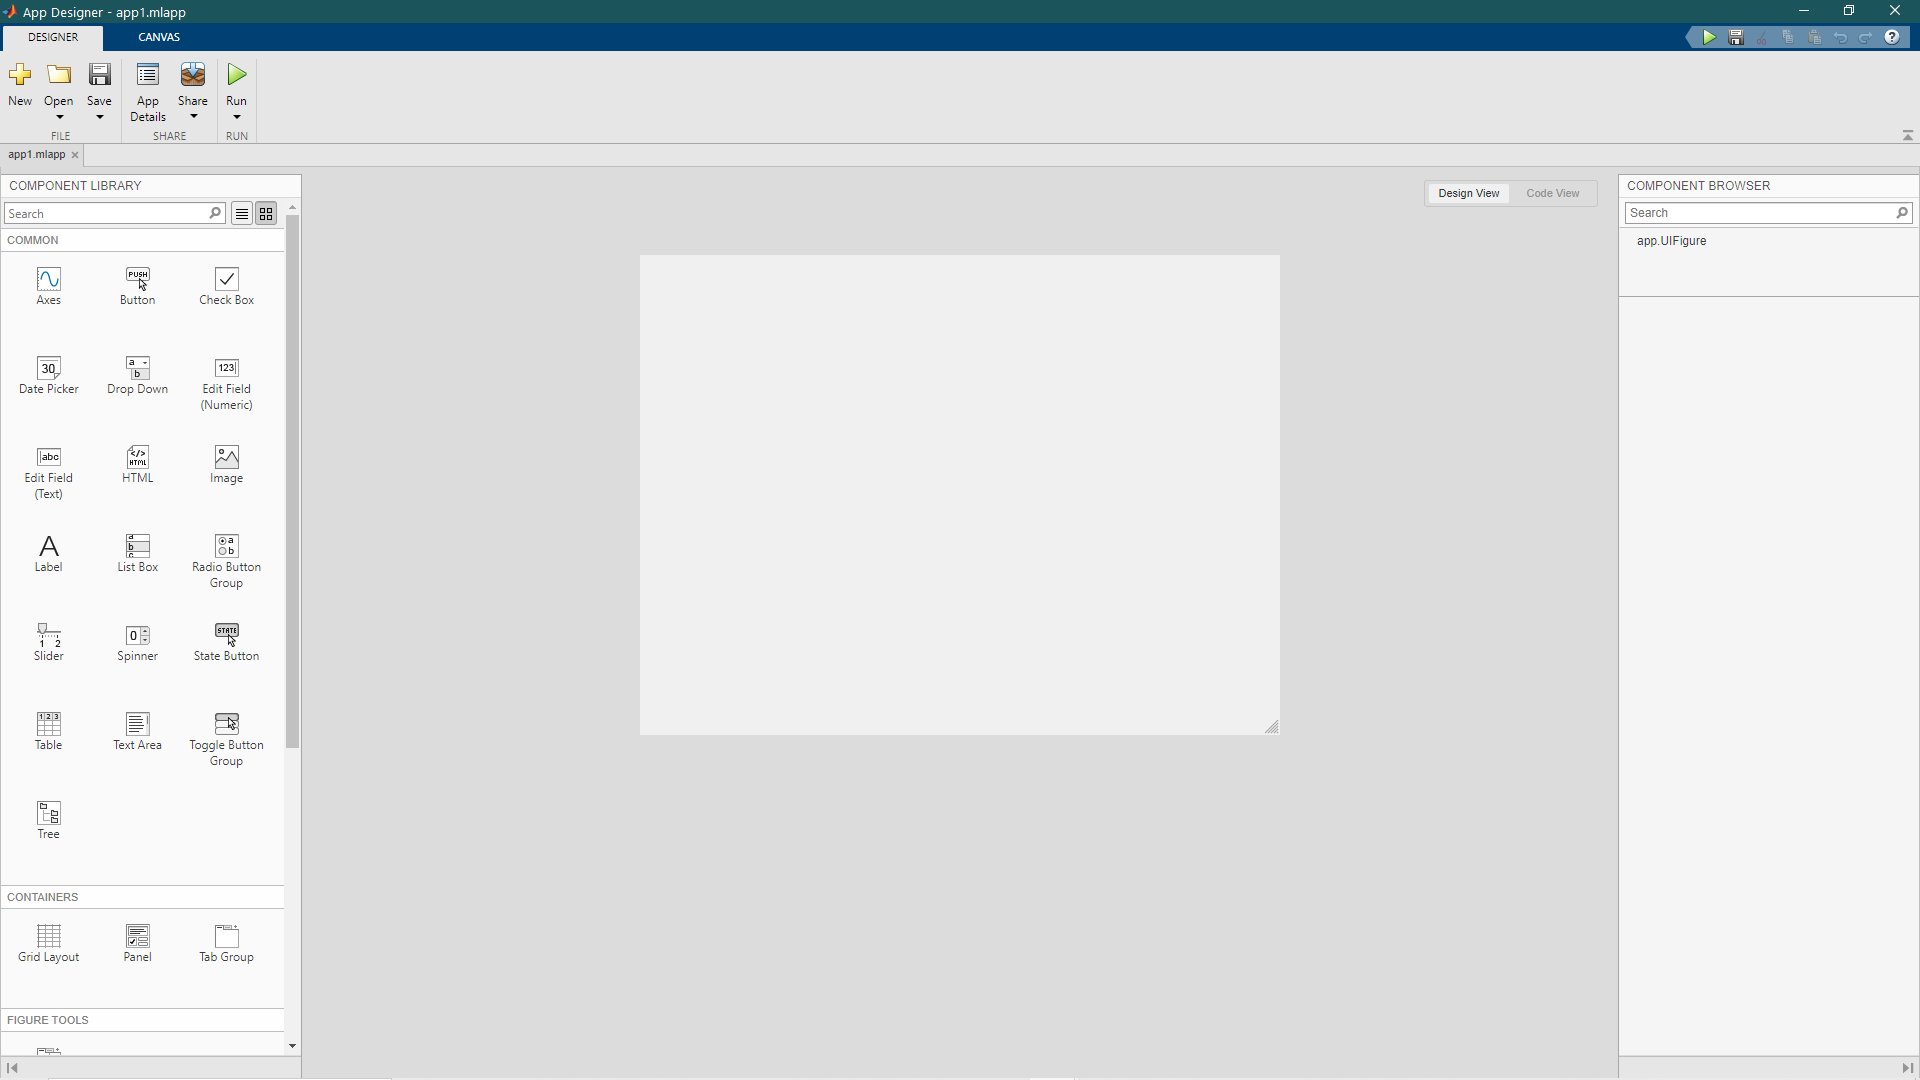
\includegraphics[width=426pt]{images/appDesignerDesignViewLayout.PNG}
    \caption{Design View Layout}
    \label{fig:designViewLayout}
\end{figure}

\subsubsection{Code View}
As you can see in Figure \ref{fig:codeViewLayout}, The Code View features two new sections along side the Component Browser. These new sections are the Code Browser and the Editor. The Editor provides access to the code which corresponds to the components that have been added to the GUI. Pre-set code that is integral to the GUI is not editable and is shown with a grey background. New sections of code that correspond to new Callbacks, Functions, and Properties are editable and are shown with a white background. These sections of code are the key to creating a functional and interactive GUI.
\begin{figure}[H]
    \centering
    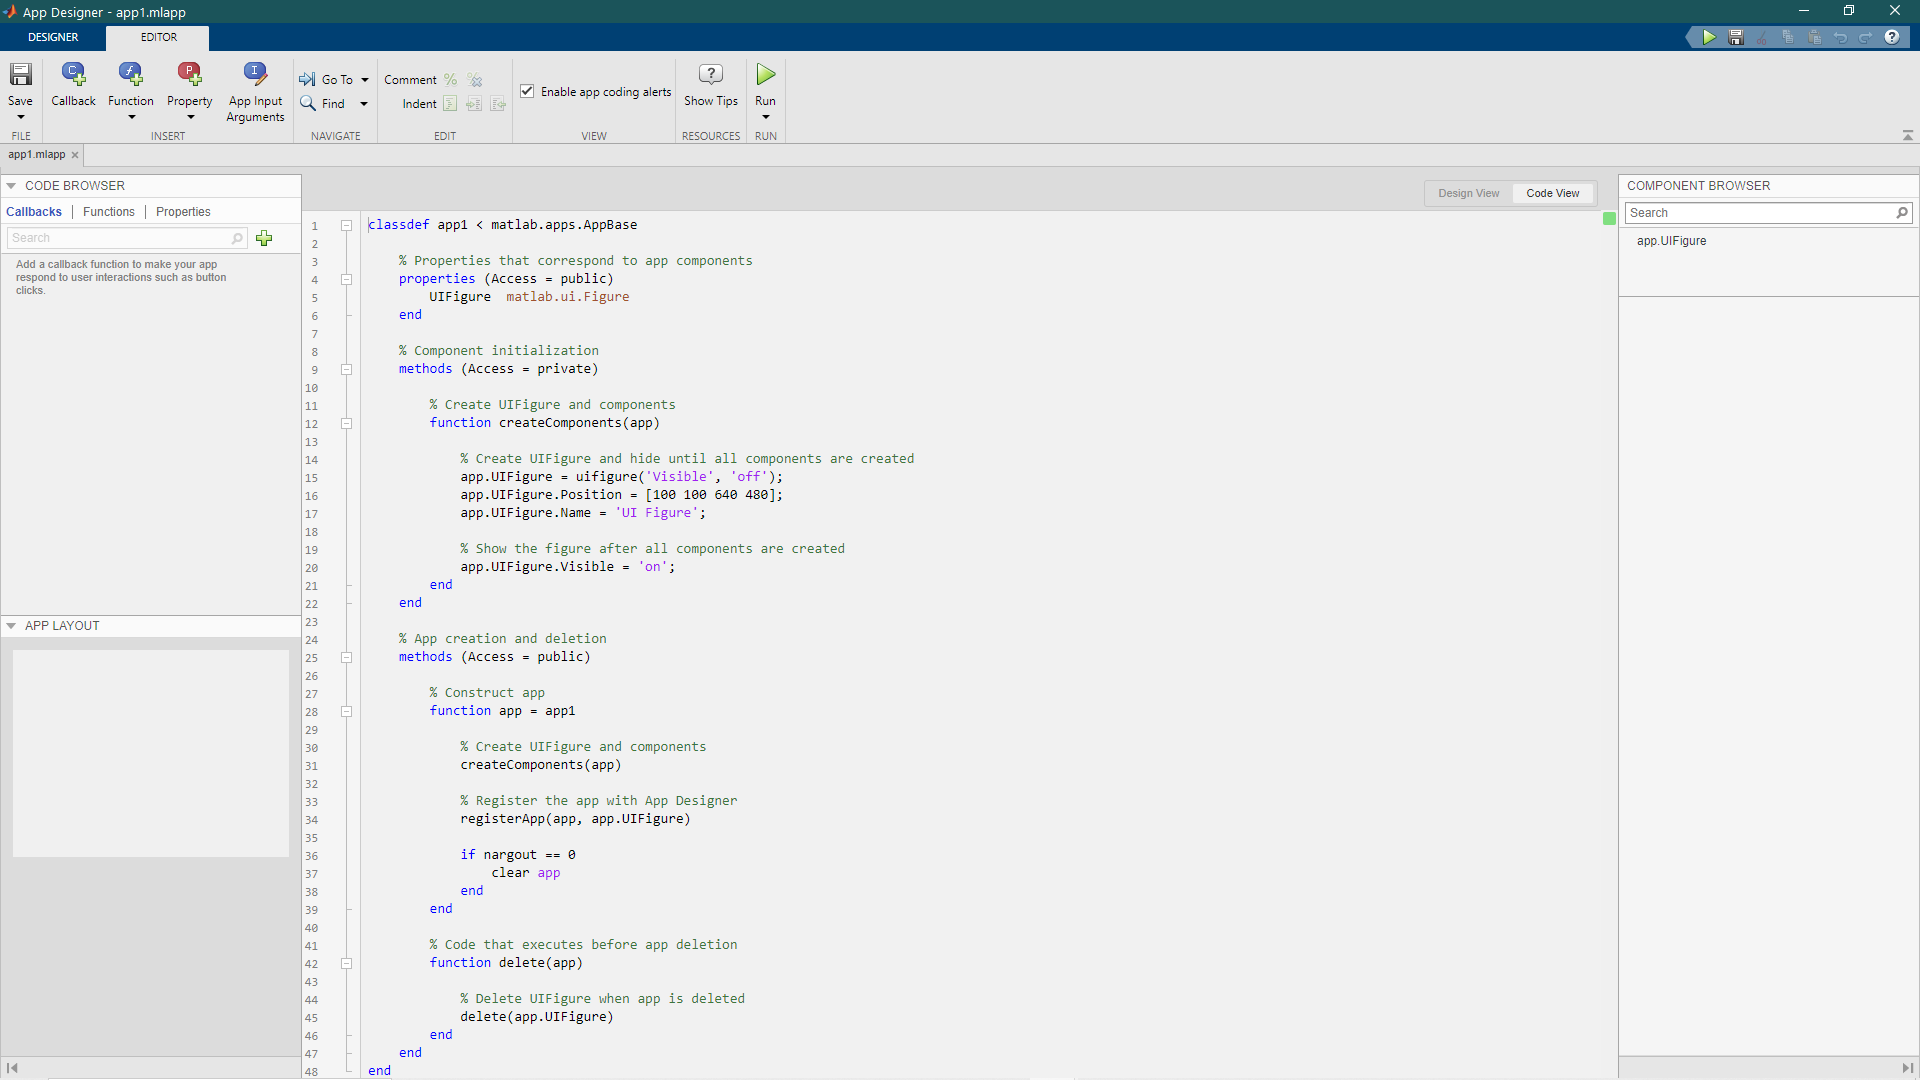
\includegraphics[width=426pt]{images/appDesignerCodeViewLayout.PNG}
    \caption{Code View Layout}
    \label{fig:codeViewLayout}
\end{figure}
\subsubsection{Callbacks}
Callbacks are used to add functionality and interactivity to components of the GUI in order to enable your app to respond to user interactions such as button clicks. Callbacks can be added through the Callbacks section of the Code Browser, the Callbacks section of the Component Browser, or by right-clicking eligible components on the Canvas.

\subsubsection{Functions}

Functions can be defined within your app so that you can call them in different places and keep your code organized. Functions can be private or public. Private functions can only be called inside the app, which makes them useful for single-window apps. Public functions can be called either inside or outside the app, which makes them useful for multi-window apps. For this project, as you will only be dealing with a single-window app, you will only be needing private functions.

\subsubsection{Properties}
Properties are used within your app to store and share data between callbacks and functions. Like functions, properties can be either private or public. Private properties store data to be shared inside the app, which makes them useful for single-window apps. Public properties store data to be shared inside or outside the app, which makes them useful for multi-window apps. For this project, as you will only be dealing with a single-window app, you will only be needing private properties.

\end{document}